
% ---
% Modelo Epidemiológico
% ---
\chapter{Modelo Epidêmico}
\label{cap:modelo_epidemico}
% ---
    A seguir, analisamos o modelo epidemiológico SIS multiplicativo, conforme apresentado em \cite{rufino2018contaminaccao}.  As Seções~\ref{sec:descrmodel} e~\ref{sec:modelbinon} descrevem o  modelo.  
    A Seção~\ref{sec:otimon} apresenta resultados sobre o estado mais provável, seguida pela  busca dos valores ótimos para parametrizar o modelo, relacionando tais valores com o estado mais provável.

	\begin{table}[!htb]
	\footnotesize
		\centering 
			\caption{Tabela de notação}
		\begin{tabular}{clc}
			\hline
			variável 		& descrição 								& valor de referência \\ 
			\hline
			$M$ 			& tamanho total da população 				& 100 \\
			$N$ 			& população passível de infecção 			& M\\
			$\gamma$ 		&  fator de infecção endógena (por aresta) 	& 1.09 \\
			$\lambda$ 		&  fator de infecção exógena (por nó) 		& $\Lambda/N$ \\ 
			$\Lambda$ 		& fator de infecção exógena total 			& 10 \\
			$A$ 			& matriz de adjacência (conexões) 			& completa \\
			$d$ 			& número de nós vizinhos infectados 		& - \\
			$\lambda \gamma^d$ &  taxa de infecção (por nó)  			& - \\
			$\mu$ 			& taxa de recuperação 						& 1 \\
			$\pi(\bm{x})$ 	& probabilidade do estado $\bm{x} $			& - \\
			$i$  			& número de nós infectados na rede 			& - \\
			$\rho$ 			& probabilidade de um nó escolhido ao acaso estar contaminado & - \\
			\hline
		\end{tabular}
 	\label{tab:notation}
	\end{table}
	
    \section{Descrição do modelo}  
    \label{sec:descrmodel}
    	Consideramos uma população finita contendo $M$ nós, dos quais, $N$ decidiram não vacinar, e portanto possuem uma vulnerabilidade que pode ser explorada.	Cada um desses $N$ nós pode assumir os estados de suscetível ($S$ ou $0$) ou infectado ($I$ ou $1$). 
    	
    	Um nó infectado pode ser recuperado, passando do estado $I$  para o estado $S$ após um tempo  exponencialmente distribuído com média 
    	$1/\mu$.
    	Um nó suscetível pode ser infectado por um atacante externo (infecção exógena) ou por um ataque interno (infecção endógena) de um vizinho na rede. Seja $d$ o número de vizinhos infectados.  
    	Seja $\gamma$ a taxa de infecção endógena por vizinho e seja $\lambda$ a taxa de infecção exógena por nó, $\lambda = \Lambda /N$.  
    	Assumimos que o tempo entre  infecções é exponencialmente distribuído, com taxa  $\gamma^d \lambda$. Ou seja, assumimos contribuições  multiplicativas das taxas de infecções endógenas e exógenas.  

    	Seja $\bx$ um estado possível da rede, entre todos os estados possíveis $\mathcal{X}$. O estado é um vetor $N$ dimensional, $\bx \in \{0,1\}^N$, $\bx=(x_1, x_2, \cdots, x_k, \cdots, x_{N-1},x_{N})$, onde $x_k \in \{0,1\}$. A dinâmica do sistema é caracterizada por um processo Markoviano contínuo, homogêneo temporal, irredutível e de estados finitos. Cada estado da rede corresponde a um estado no processo Markoviano. Além disso, o nosso processo Markoviano é reversível, conforme \cite{kelly1979reversibility}.

    	Consideramos uma topologia totalmente conectada, onde todos os nós estão conectados entre si. A probabilidade do estado $\bx$ é dada por $\pi(\bx)$, derivada em~\cite{zhang2017contact},
    	\begin{eqnarray}
    	    \pi(\bx) & = & \frac{\tilde{\pi}(\bx)}{Z} \label{eq:equilibriumBasicScaledSIS}
    	\end{eqnarray}
	    onde
        \begin{equation}
            \tilde{\pi}(\bx)=\left( \frac{\lambda}{\mu}\right)^{1^{T}\bx} \gamma^{\bx^{T}A\bx/2} \textrm{ , } \bx \in \mathcal{X}, \qquad 	  Z= \sum_{\bx \in \mathcal{X}} \tilde{\pi}(\bx). \label{eq:equilibriumNumeratorScaledSIS}
        \end{equation}
        A Tabela~\ref{tab:notation} resume a notação.  

        Tomando proveito da simetria do problema, e com certo abuso de notação, seja $\pi(\iota)$ a probabilidade de haver $\iota$ nós infectados:
        \begin{equation}
            \pi(\iota) = \frac{\tilde{\pi}(\iota)}{Z}, \qquad \tilde{\pi}(\iota) = \binom{N}{\iota} \left(\frac{\lambda(N)}{\mu}\right)^{\iota} \gamma^{\iota(\iota-1)/2}, \quad \iota=0, \ldots, N.  \label{eq:scaledSISProbIotaInfected}
        \end{equation}

	    O valor esperado do número de nós infectados é
    	\begin{equation}
    	    E(I) = \sum\limits_{\iota = 0}^{N} \iota \frac{\tilde{\pi}(\iota)} {Z} = N\rho(N), \quad \rho(N) = \frac{1}{N} \sum\limits_{\iota = 0}^{N} \iota \frac{\tilde{\pi}(\iota)}{Z} \label{eq:scaledSIS_espected_infecteds}
    	\end{equation}
	    onde $\rho(N)$	é a probabilidade de  infecção de um nó escolhido aleatoriamente. 

    \section{Aproximação binomial} \label{sec:modelbinon}
	    A análise direta das equações acima é complexa, por envolver um termo quadrático no expoente de $\gamma$ em \eqref{eq:scaledSISProbIotaInfected}.  Para simplificar a análise, consideramos  uma solução aproximada. Para tal, definimos $\hat\rho(N) \approx \rho(N)$ e $\hat\pi(\iota) \approx \tilde\pi(\iota)$:
		\begin{align}
		  \hat {\rho}(N)	&=  \frac{1}{N} \sum\limits_{\iota=0}^{N}\iota \frac{\hat{\pi}(\iota)}{{\hat Z}}, \quad \hat{Z} = \sum\limits_{\iota=0}^{N} \hat{\pi}(\iota), \quad \hat{\pi}(\iota)	=  \binom{N}{\iota} \left(\frac{\lambda(N)}{\mu}\gamma^{N^{\star}}\right)^{\iota}\label{eq:rho_Nhat1} 
		\end{align}
		onde $N^{\star}(N)$ é uma função crescente de $N$, que denotamos simplesmente por $N^{\star}$ para simplificar a notação.  Nos referimos ao modelo proposto para aproximar a solução do modelo original como \emph{modelo binomial}, por fazermos uso do binômio de Newton na demonstração do resultado a seguir. 

		\begin{lemma}
			No modelo binomial,  temos que:
				\begin{equation}
							\hat{\rho}(N) =   \frac{1}  {1+ \mu/(\lambda(N) \gamma^{N^{\star}} )  }  \label{eq:mainlema} %\tag{3} \label{e}
				\end{equation} 
		\end{lemma}	

		A demonstração do lema acima consta em  \cite{rufino2018contaminaccao}, notando o pequeno ajuste de notação na nova versão do resultado, refletindo a nova definição de $N^{\star}$.

	    Como discutido na Seção~\ref{sec:otimon} a seguir, $N^{\star}$ é adequadamente parametrizado como $N^{\star} = (N-1)\hat{\rho}(N)$. Simplificando a notação,  removendo as dependências  com relação a $N$,

		\begin{equation}
			\hat{\rho} =   \frac{1}  {1+ \mu/(\lambda \gamma^{(N-1)\hat{\rho}} )  }  \label{eq:mainlema1} %\tag{3} \label{e}
		\end{equation} 
	    A equação acima dá origem a um problema de ponto fixo, analisado na Seção~\ref{sec:fechada}.

        \begin{figure}[!htb]
    		\centering
    	    \hspace{-0.2in}	
            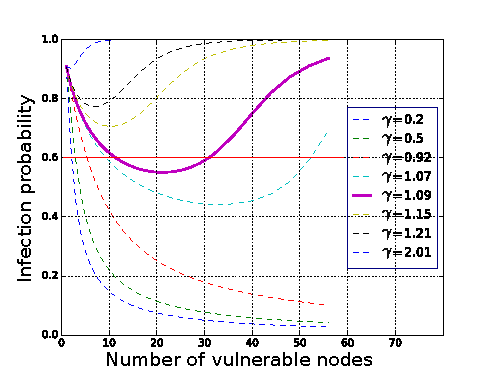
\includegraphics[width=0.49\columnwidth,keepaspectratio=true]{./img/scaled_sis_lambda_10_EN_curves.pdf}
    		\caption{Equilíbrio em relação as motivações para vacinar ou não vacinar ($\gamma=1,09$).}
    		\label{fig:equilibrim_cost}
        \end{figure}


	\section{Buscando valor ótimo para  \texorpdfstring{$N^{\star}$}{N*}}
	\label{sec:otimon}
		A seguir, buscamos o valor ótimo de $N^{\star}$ em função de $N$.  Para tal, nos aproveitamos de um resultado recentemente derivado em~\cite{zhang2018more} sobre os estados mais prováveis do modelo epidemiológico  aqui discutido. Em~\cite{zhang2018more}, os autores discutem o cenário no qual  a taxa de infecção exógena, $\lambda$, é constante, independente de $N$.   Reproduzimos o principal resultado de~\cite{zhang2018more}, tendo em vista que ele  nos traz \emph{insights} sobre o valor ótimo de $N^{\star}$. 

		Seja $\bx^{\star}$ a \textit{configuração mais provável} do sistema,  $\bx^{\star} = [x_1^{\star}, x_2^{\star}, \ldots, x_{N}^{\star}]$, onde $\bx^{\star} = \argmax\limits_{\bx \in \mathcal{X}} \: \pi(\bx)$. 
		Se $\tilde{\pi}(\bx^{\star}) \gg \tilde{\pi}(\bx)$ , $\forall \bx \in \mathcal{X}\slash \bx^{\star}$, então 
        \begin{equation}
        	P(x_{k} =1) \approx  \frac{1}{1+\mu/\left(\lambda\gamma^{m_{k}^{\star}}\right)}, \quad \textrm{, onde }  m_{k}^{\star}=\sum\limits_{j=1}^{N} a_{kj}x_{j}^{\star}. \label{eq:aproximacao_Zhang}
        \end{equation}
		O resultado acima decorre do fato de que a probabilidade do estado $\bx$ pode ser expressa como $\pi(\bx)=e^{H(\bx)}$, onde $H(\bx)=1^{T} \bx \: \log \left( {\lambda}/{\mu} \right) + \left( \bx^{T} A \bx \: \log \gamma\right) /2$.  Notando então a  relação entre $\pi(\bx)$ e a distribuição de Gibbs, o resultado segue.
        
		Note que  $m_{k}^{\star}$ representa o números de vizinhos de $k$  contaminados no estado mais provável. Comparando~\eqref{eq:aproximacao_Zhang} e~\eqref{eq:mainlema}, vemos que $m_{k}^{\star}$ está  diretamente relacionado a $N^{\star}$.  
		Seja $n$ o número de vizinhos de um nó típico.  Ao considerarmos um  grafo completo, o número de vizinhos de cada nó é $n=N-1$, e o número médio de vizinhos contaminados é $\rho n$.  Substituindo $N^{\star}$ em~\eqref{eq:mainlema} por $m_k^{\star}$,  obtemos então a expressão~\eqref{eq:aproximacao_Zhang}.
		Tal argumento sugere que o valor ótimo de $N^{\star}$ é dado por $N^{\star}=\hat{\rho}  n$.   A seguir, ilustramos numericamente tal fato.

		A Figura~\ref{fig:result_01b} ilustra como  a probabilidade de infecção  em função do número de nós não vacinados na rede, $N$. Consideramos $\lambda=\Lambda/N$, $\Lambda=10$, $\mu=1$ e $\gamma=1.09$.   O valor de $\hat{\rho}$ obtido via aproximação, quando selecionamos o melhor valor de $N^{\star}$, é muito próximo do valor de $\rho$ exato.  A Figura~\ref{fig:result_01b}(a) mostra também que quando fazemos $N^{\star}=N$ e $N^{\star}=N/2$ obtemos limites superiores e inferiores para a probabilidade de contaminação. Para avaliar a qualidade da aproximação $N^{\star}=\rho (N-1)$, a Figura~\ref{fig:result_01b}(b) mostra o valor ótimo de $N^{\star}$, em função de $N$, comparado com $N/2$, $\rho N$ e $\rho (N-1)$. Tanto $\rho N$ quanto $\rho (N-1)$ apresentam excelentes aproximações.  Calculando a soma dos erros quadráticos (em destaque na figura), podemos identificar que de fato $\rho(N-1)$ é uma melhor aproximação, corroborando os resultados derivados nessa seção. 
		

    \section{Fórmulas fechadas via método de Newton}
    \label{sec:fechadageral}
    	A seguir indicamos como usar o método de Newton para achar fórmulas fechadas aproximadas para~\eqref{eq:mainlema}.
	    Pelo fato de $\rho$ aparecer tanto do lado direito quanto do lado esquerdo de~\eqref{eq:mainlema}, a equação não é passível de solução exata em fórmula fechada.  Ao invés de buscar por soluções exatas, buscamos então por aproximações. Para tal, vamos considerar as seguintes funções auxiliares, 
    	\begin{eqnarray}
    		f(\rho)		&=& 	\rho \left( 1 + \frac{\mu}{\lambda}\gamma^{-\rho n} \right) -1  =  
    							\rho + \rho \frac{\mu}{\lambda} \gamma^{-\rho n} -1 \label{eq:2} \\
    		\frac{ \partial{f(\rho)}}{ \partial \rho}  = 
    		f'(\rho)	&= &	1 + \frac{\mu}{\lambda} \gamma^{-\rho n} 
    							\left( 1 - \rho n \ln \gamma \right)  \label{eq:3} \\
    		\frac{\partial^2{f(\rho)}}{ \partial^2 \rho}  = 
    		f''(\rho)	&= & 	g \frac{\mu \ln \gamma}{\lambda} \gamma^{-\rho n} 
    							\left( \rho (\ln \gamma) -2 \right)  \label{eq:4}
    	\end{eqnarray}
    	Encontrar a solução $\rho$ para~\eqref{eq:mainlema1} é equivalente a encontrar as raízes (i.e., os zeros) de~\eqref{eq:2}.

	    A iteração  do método de Newton, adaptada ao nosso cenário, é dada por,
	    \begin{equation}
	        \rho_{i+1} =  \rho_{i} - \frac{f(\rho_{i})}{f'(\rho_{i})} = \frac{\lambda-\mu\gamma^{-\rho_{i}n} \left(\rho_{i}^{2} n\ln\gamma\right)}{\lambda-\mu \gamma^{-\rho_{i}n} \left(\rho_{i}n \ln\gamma-1\right)} \label{eq:newton_general}
	    \end{equation}
	    Destacamos que $f(0)=-1$ e $f(1) = \frac{\mu}{\lambda \gamma} > 0$, onde $ \mu, \lambda > 0$ e $\gamma > 1$.  Além disso, $f(0)=-1$ e $ f'(0) =  {\mu}/({\lambda \gamma})$, assim como $ f''(0) = {\mu \ln \gamma}/{\lambda}$.  Desta forma, se $\gamma > 1$, então $f(0)  f''(0) > 0$ ($f$ e $f''$ têm o mesmo sinal). Pelo teorema  de  Darboux \cite{mikusinski1955methode}, iniciando com  $\rho_0 = 0$, o método de Newton converge sem  ultrapassar (\emph{overshoot}) a solução.


	\section{Obtendo fórmulas fechadas}
	\label{sec:fechada}
		Usando a abordagem descrita acima, obtemos  fórmulas fechadas para uma aproximação da probabilidade de um nó estar infectado.  Numericamente, identificamos que considerar  duas iterações do método de Newton é suficiente para obter boas aproximações.

		A condição inicial do método de Newton tem um papel importante no resultado.  Consideramos então duas condições iniciais extremas. Seja $\rho_0$ a condição inicial do método.  Considerando $\rho_0=0$ e $\rho_0=1$, obtemos duas aproximações para a probabilidade de contaminação.  Na próxima seção, apresentamos uma heurística simples para determinar quando adotar uma condição inicial ou a outra.  Na Seção~\ref{sec:fechadageral}, indicamos numericamente que as aproximações junto com a heurística capturam o comportamento da probabilidade de infecção.

		Seja $\rho_i^{(0)}$ a probabilidade de infecção aproximada após $i$ iterações do método de Newton, com condição inicial $\rho_0=0$. Então, 
			 \begin{eqnarray}
			  \rho_{0}^{(0)} &=& 0, \quad \rho_1^{(0)} = \frac{\lambda}{\lambda + \mu}   \nonumber \\
			  \rho_{2}^{(0)} &=& \frac{ \lambda - \mu \gamma^{-\rho_{1} n }  \left( \rho_{1}^{2} n  \ln \gamma    \right) }  
		                            { \lambda - \mu \gamma^{-\rho_{1} n }  \left( \rho_{1}     n  \ln \gamma  -1 \right) } \nonumber =  \frac{ \lambda - \mu \gamma^{-\left( \frac{\lambda}{\lambda + \mu} \right) n }  \left( \left( \frac{\lambda}{\lambda + \mu} \right)^{2} n  \ln \gamma    \right) }  
		                            { \lambda - \mu \gamma^{-\left( \frac{\lambda}{\lambda + \mu} \right) n }  \left( \left( \frac{\lambda}{\lambda + \mu} \right)     n  \ln \gamma  -1 \right) } \label{eq:rho_2iter_rho0_0}
			 \end{eqnarray}

		Analogamente, seja $\rho_i^{(1)}$ a probabilidade de infecção aproximada após $i$ iterações do método de Newton, com condição inicial $\rho_0=1$. Então, 
 
    	\begin{equation}
    	  \rho_2^{(1)}    = \frac{ \lambda - \mu \gamma^{-\left( \frac{ \lambda - \mu \gamma^{- n }  \left( n  \ln \gamma    \right) }  { \lambda - \mu \gamma^{- n }  \left( n  \ln \gamma  -1 \right) }  \right) n } \left( \left( \frac{ \lambda - \mu \gamma^{- n }  \left( n  \ln \gamma    \right) }  { \lambda - \mu \gamma^{- n }  \left( n  \ln \gamma  -1 \right) }  \right)^{2} n \ln \gamma \right) }  
    		                    { \lambda - \mu \gamma^{-\left( \frac{ \lambda - \mu \gamma^{- n }  \left( n  \ln \gamma    \right) }  { \lambda - \mu \gamma^{- n }  \left( n  \ln \gamma  -1 \right) }  \right) n } \left( \left( \frac{ \lambda - \mu \gamma^{- n }  \left( n  \ln \gamma    \right) }  { \lambda - \mu \gamma^{- n }  \left( n  \ln \gamma  -1 \right) }  \right)     n \ln \gamma -1 \right) } 
    		                    \label{eq:rho_2iter_rho0_1}
    	\end{equation}
	    A fórmula fechada com $\rho_0=0$ é bem mais simples que com $\rho_0=1$. Conforme iremos indicar nas seções a seguir, para muitos cenários a primeira aproximação, mais simples, é suficiente.  


    	\subsection{Heurística para determinação da condição inicial}
	    \label{subsec:heuristica}
    	A seguir consideramos uma heurística para determinar a condição inicial ótima da iteração de Newton descrita na seção anterior.  Para tal, ilustramos o comportamento da aproximação quando $\rho_0=0$ na Figura~\ref{fig:rho_exact_approx_newton_rho0_0e1}(a) e $\rho_0=1$ na Figura~\ref{fig:rho_exact_approx_newton_rho0_0e1}(b) exceto a curva para $\gamma=1.03$, usando os valores referência na Tabela~\ref{tab:notation}. % Os demais valores, quando não for explicitamente dito, usaremos os valores de referência da Tabela~\ref{tab:notation}. 
    	Na medida em que $N$ aumenta, a condição inicial $\rho_0=1$ tende a produzir melhores aproximações.  Entretanto, para valores pequenos de $\gamma$ (e.g., $\gamma=1,03$) é preciso utilizar a condição inicial $\rho_0=0$ mesmo para valores grandes de $N$.

    	\begin{figure}[!htb]
    	    \centering
    	    \begin{tabular}{cc}
    	         \hspace{-1.2cm}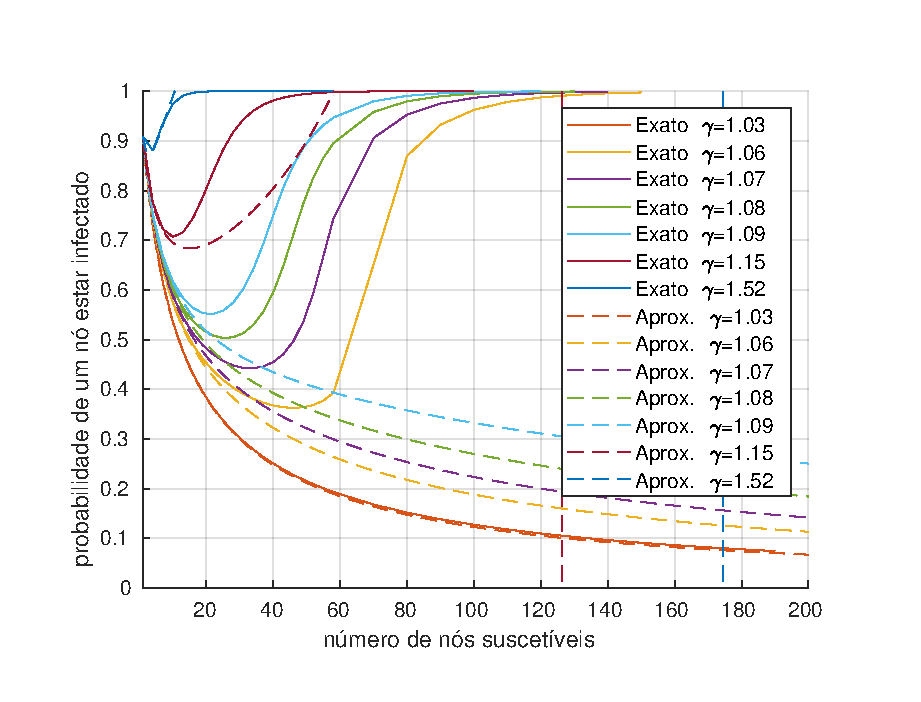
\includegraphics[width=0.6\columnwidth]{img/exact_approx_v0_lambda10_00_gamma1_52_iter_2_rho0_0.pdf}&
    	         \hspace{-1.2cm}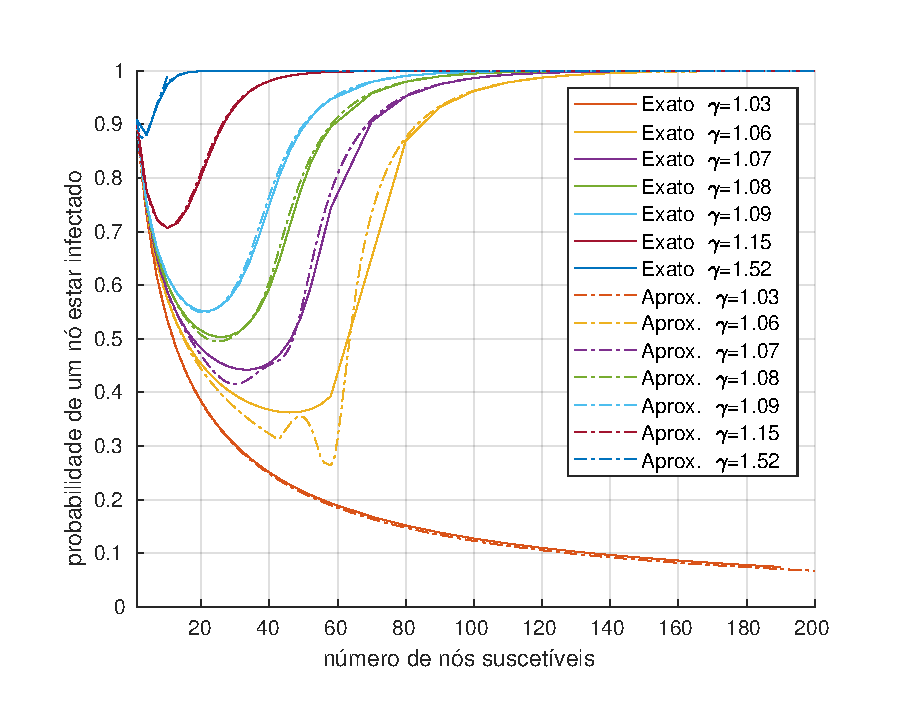
\includegraphics[width=0.6\columnwidth]{img/exact_approx_lambda10_00_gamma1_52_iter_2.pdf}\\
    	         \hspace{-1.2cm}(a) $\rho_{0}=0$ & \hspace{-1.2cm}(b) $\rho_{0}$ dado por~\eqref{eq:heuri} 
    	    \end{tabular}
    	   \caption{Probabilidade de infecção, calculada usando método de Newton com (a)  condição inicial $\rho_0=0$ e (b) heurística para condição inicial.}
    	    \label{fig:rho_exact_approx_newton_rho0_0e1}
    	\end{figure}

        Dependendo da condição inicial, o método de Newton pode  convergir para valores maiores que 1 ou menores que 0. Como ilustrado na Figura~\ref{fig:rho_exact_approx_newton_rho0_0e1}(a),  para $\gamma=1,52$ e $1,15$. Portanto, nossa  heurística para determinar  a  inicialização parte da definição das seguintes quantidades auxiliares adicionais,
        \begin{equation}
    	    \bar{\rho}_2^{(z)}(N) = \left\{
            \begin{array}{ll}
                {\rho}_2^{(z)}(N), & \textrm{se } 0 \leq {\rho}_2^{(z)}(N) \leq 1 \textrm{ e } \bar{\rho}_2^{(z)}(N-1) \neq -\infty, \\
    	        -\infty, & \textrm{caso contrário.}
            \end{array}\right. \label{eq:condi}
    	\end{equation}
	    onde $z$ é a condição inicial, $0 \leq z \leq 1$.
	    Segundo~\eqref{eq:condi}, se o método de Newton convergir para valores além do domínio de interesse para determinada condição inicial, tal condição é descartada daí em diante.  Em~\eqref{eq:condi} deixamos explícita a dependência de $\rho$ com relação a $N=n+1$ (na Seção~\ref{sec:fechada} tal dependência foi mantida implícita). Motivado pela discussão acima, nossa heurística é então dada por,
    	\begin{equation} \label{eq:heuri}
    	    \bar{\rho}(N) = \max(\bar{\rho}_2^{(0)}(N), \bar{\rho}_2^{(1)}(N))
    	\end{equation}
	    A Figura~\ref{fig:rho_exact_approx_newton_rho0_0e1}(b) ilustra a qualidade das aproximações obtidas por meio da heurística de inicialização. Para os cenários em consideração a heurística foi capaz de determinar boas escolhas para inicializar os parâmetros. 

	\section{Vacinar, reiniciar ou esperar?}
	    Tendo em vista a solução com fórmulas fechadas descrita nesta seção, podemos gerar curvas como aquela apresentada na Figura~\ref{fig:rho_exact_approx_newton_rho0_0e1} de forma bem eficiente.  Dada esta curva, assumimos então um custo fixo da contramedida mais custosa (vacinar).  Para fins de ilustração, consideramos que o custo é dado pela  probabilidade de um nó estar infectado. % Por exemplo, o custo pode refletir  a probabilidade de ocorrer uma catástrofe. 
	    A utilidade do usuário é dada então pela diferença entre a probabilidade de infecção  e o custo.   Considere, por exemplo, o caso $\gamma=1,07$ na Figura~\ref{fig:rho_exact_approx_newton_rho0_0e1} e o custo igual a $0,5$.  Segundo a Figura~\ref{fig:rho_exact_approx_newton_rho0_0e1}, se o número de nós não vacinados for menor ou igual a 20, a probabilidade de infecção é alta e os nós tem incentivos para se vacinarem (sistema dominado por infecções exógenas).  Por outro lado, se o número de nós não vacinados variar entre 20 e 50, o custo de vacinação é superior à probabilidade de infecção. Nesse caso,  os nós tem incentivo para não vacinarem-se, e simplesmente esperarem e reiniciarem suas máquinas quando detectarem um ataque (de forma reativa) ou quando avaliarem que o sistema está ocioso (de forma proativa).   

	    \textbf{Mensagem desta seção} Nesta seção, apresentamos fórmulas fechadas para estimar a probabilidade de contaminação de nós na rede.  As fórmulas fechadas podem ser usadas para guiar a tomada de decisão com relação a contramedidas (e.g., vacinar, reiniciar ou esperar, conforme discutido acima).  Na seção a seguir, indicamos por meio de simulações que de fato os regimes discutidos acima, nos quais diferentes contramedidas são adotadas, também são observados nos cenários simulados.  

